\documentclass[margin=5mm]{standalone}
\usepackage[dvipsnames]{xcolor}
\usepackage{pgfplots}
\usepackage{tikz}
\usepackage[tikz]{ocgx2}

\pgfplotsset{compat=1.18}
\begin{document}

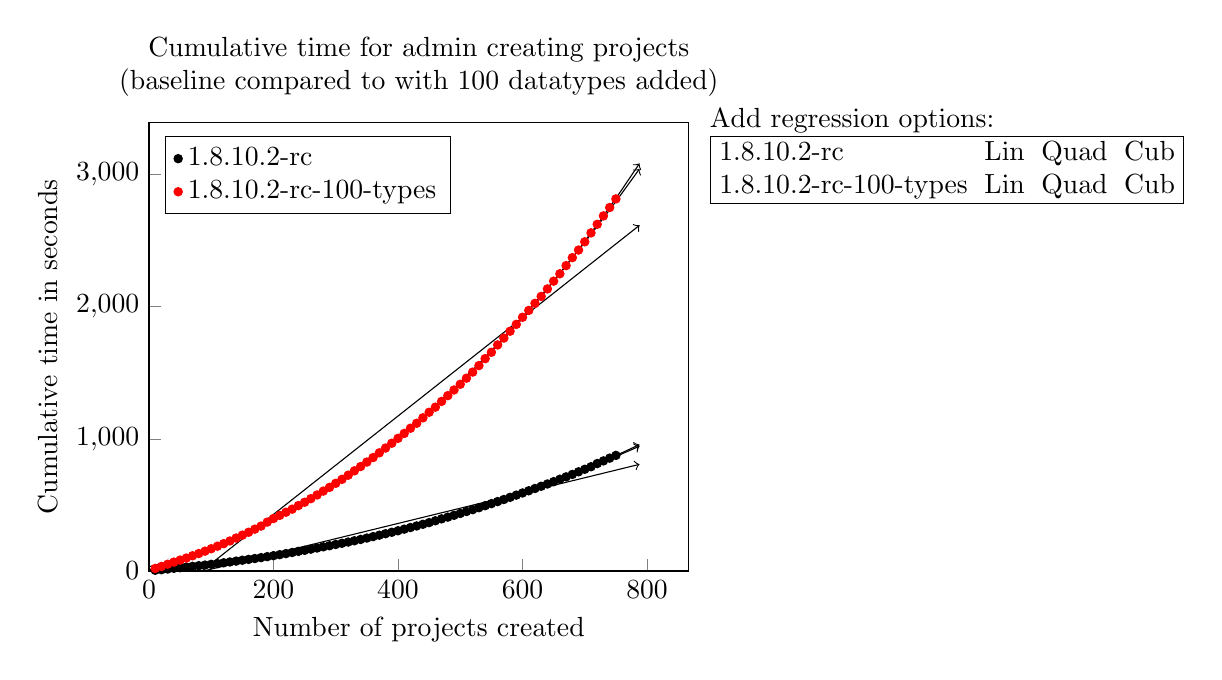
\begin{tikzpicture}
    \begin{axis}[
        align = center,
        legend pos = north west,
        legend cell align = left,
        xlabel = Number of projects created,
        ylabel = Cumulative time in seconds,
        xtick pos = left,
        ytick pos = left,
        scaled ticks = false,
        xmin = 0,
        ymin = 0,
        title = {Cumulative time for admin creating projects (baseline compared to with 100 datatypes added)},
        title style = {text width = 0.8\textwidth},
        legend entries={\switchocg{1.8.10.2-rc}{1.8.10.2-rc},\switchocg{1.8.10.2-rc-100-types}{1.8.10.2-rc-100-types}}]
        \begin{scope}[ocg = {ref = 1.8.10.2-rc-Lin, status = invisible}]
            \plot[domain=0:788,->,forget plot] (\x,{-101.71050882882894939029938541352748870849609375 + 1.1527960056899007046382621410884894430637359619140625*(\x)^1});
        \end{scope}
        \begin{scope}[ocg = {ref = 1.8.10.2-rc-Quad, status = invisible}]
            \plot[domain=0:788,->,forget plot] (\x,{10.19560248796711476870768819935619831085205078125 + 0.28080033309148955122935831241193227469921112060546875*(\x)^1 + 0.00114736272710317288754666709138518854160793125629425048828125*(\x)^2});
        \end{scope}
        \begin{scope}[ocg = {ref = 1.8.10.2-rc-Cub, status = invisible}]
            \plot[domain=0:788,->,forget plot] (\x,{1.9313749705866085637495643823058344423770904541015625 + 0.407123939823063218934606766197248362004756927490234375*(\x)^1 + 0.0007345641498114397795193841744776364066638052463531494140625*(\x)^2 + 0.00000036210401516818702008330965735893869350547902286052703857421875*(\x)^3});
        \end{scope}
        \begin{scope}[ocg = {ref = 1.8.10.2-rc, status = visible}]
            \addplot[
                only marks,
                color = black,
                mark = *,
                mark size = 1.5 pt
            ]coordinates {(10,5.234)(20,9.554)(30,14.591)(40,20.063)(50,24.849)(60,29.689)(70,34.462)(80,39.704)(90,44.62)(100,50.145)(110,55.578)(120,61.589)(130,67.877)(140,74.301)(150,81.008)(160,87.37)(170,93.995)(180,100.868)(190,108.185)(200,115.531)(210,123.127)(220,131.31)(230,139.584)(240,148.214)(250,156.376)(260,164.98)(270,173.544)(280,182.47)(290,190.803)(300,200.26)(310,209.463)(320,218.83)(330,228.454)(340,238.447)(350,248.949)(360,259.936)(370,270.547)(380,281.687)(390,292.708)(400,304.036)(410,316.268)(420,328.559)(430,340.462)(440,353.201)(450,365.832)(460,379.701)(470,394.098)(480,407.262)(490,420.961)(500,435.084)(510,449.827)(520,463.801)(530,478.391)(540,493.776)(550,509.289)(560,524.887)(570,540.43)(580,557.004)(590,573.582)(600,589.944)(610,606.709)(620,623.827)(630,640.534)(640,657.912)(650,675.509)(660,693.888)(670,711.872)(680,730.181)(690,750.057)(700,769.205)(710,788.405)(720,812.701)(730,832.729)(740,853.409)(750,874.163)};
        \end{scope}
        \begin{scope}[ocg = {ref = 1.8.10.2-rc-100-types-Lin, status = invisible}]
            \plot[domain=0:788,->,forget plot] (\x,{-315.94937117117120806142338551580905914306640625 + 3.7202564153627317722339284955523908138275146484375*(\x)^1});
        \end{scope}
        \begin{scope}[ocg = {ref = 1.8.10.2-rc-100-types-Quad, status = invisible}]
            \plot[domain=0:788,->,forget plot] (\x,{32.228962828581558142104768194258213043212890625 + 1.00717848809193011305751497275196015834808349609375*(\x)^1 + 0.00356983937798789792428255651657309499569237232208251953125*(\x)^2});
        \end{scope}
        \begin{scope}[ocg = {ref = 1.8.10.2-rc-100-types-Cub, status = invisible}]
            \plot[domain=0:788,->,forget plot] (\x,{4.19717161545090267082969148759730160236358642578125 + 1.4356610004310310646502557574422098696231842041015625*(\x)^1 + 0.0021696500067026375409284799644638042082078754901885986328125*(\x)^2 + 0.00000122823629060110633501464415251458461852962500415742397308349609375*(\x)^3});
        \end{scope}
        \begin{scope}[ocg = {ref = 1.8.10.2-rc-100-types, status = visible}]
            \addplot[
                only marks,
                color = red,
                mark = *,
                mark size = 1.5 pt
            ]coordinates {(10,18.846)(20,33.866)(30,50.842)(40,66.995)(50,82.289)(60,97.567)(70,114.873)(80,131.805)(90,149.785)(100,168.07)(110,187.222)(120,206.52)(130,226.667)(140,248.915)(150,270.784)(160,292.791)(170,316.247)(180,339.449)(190,369.742)(200,396.668)(210,420.422)(220,444.213)(230,467.455)(240,494.366)(250,519.81)(260,546.884)(270,574.807)(280,604.134)(290,632.371)(300,663.131)(310,693.1)(320,724.517)(330,757.681)(340,790.036)(350,823.922)(360,858.004)(370,893.854)(380,929.926)(390,966.216)(400,1003.342)(410,1040.459)(420,1079.759)(430,1117.403)(440,1158.532)(450,1200.672)(460,1239.204)(470,1282.895)(480,1326.305)(490,1369.25)(500,1412.393)(510,1458.421)(520,1504.618)(530,1553.677)(540,1606.398)(550,1654.55)(560,1710.077)(570,1761.874)(580,1813.752)(590,1865.66)(600,1919.395)(610,1970.919)(620,2024.561)(630,2077.119)(640,2133.819)(650,2192.551)(660,2248.455)(670,2310.135)(680,2370.484)(690,2427.919)(700,2490.235)(710,2557.894)(720,2622.668)(730,2686.392)(740,2749.683)(750,2814.843)};
        \end{scope}
    \end{axis}
    \begin{scope}
        \addtolength{\tabcolsep}{-0.3em}
        \node [below right, shape=rectangle, align=left](regressiontable) at (7,6) {
            Add regression options: \\
            \begin{tabular}{|llll|}
                \hline
                1.8.10.2-rc & \switchocg{1.8.10.2-rc-Lin}{Lin} & \switchocg{1.8.10.2-rc-Quad}{Quad} & \switchocg{1.8.10.2-rc-Cub}{Cub} \\
                1.8.10.2-rc-100-types & \switchocg{1.8.10.2-rc-100-types-Lin}{Lin} & \switchocg{1.8.10.2-rc-100-types-Quad}{Quad} & \switchocg{1.8.10.2-rc-100-types-Cub}{Cub} \\
                \hline
            \end{tabular}
        };
    \end{scope}
\end{tikzpicture}

\end{document}